\documentclass[discrete.tex]{subfiles}

\begin{document}
  \section{Код Шеннона-Фано. Алгоритм Хаффмена. 3 леммы}

  \begin{definition}
    Код называется префиксным, если никакая последовательность не является началом другой (код Шеннона-Фано). Такое св-во называется св-ом префикса
  \end{definition}

  \begin{task}
    Пусть в тексте n символов, частота появления каждого $p_i = \frac{n_i}{n}$. Можно кодировать символы последовательностью 0 и 1. Пусть соответствующая полученная длина $s_i$, $\sigma_i = \sum_i p_i s_i$. Задача $\sigma \ra \min$ по всем наборам длин. $\{s_i\}$, удовлетворяющая неравенству Крафта (необходимое и достаточное условие префиксного кода в r-ичном алфавите для данных символов) $\sum r^{-s_i} \leq 1$
  \end{task}

  \begin{definition}
    Набор, для которого $\sigma$ минимальна называется оптимальным
  \end{definition}

  \begin{sol}[Шеннона-Фано]
    Разбить все символы на две группы с примерно одинаковыми суммарными вероятностями, коды первой начать с 0, второй с 1. Внутри каждой группы сделать то же самое. Полученный код будет близок к минимальному
  \end{sol}

  \begin{sol}[решение Хаффмена]
    Основывается на трех леммах о наборе $\{s_i\}$:
    \begin{lemma}[1]
      Пусть $\{p_i\}$ - набор вероятностей символов и $\{s_i\}$ - длины оптимальных кодовых комбинаций. Если $p_1 \geq ... \geq p_n$, то $s_1 \leq ... \leq s_n$
    \end{lemma}

    \begin{proof}
      По задаче о перестановке, минимизирующей скалярное произведение двух векторов
    \end{proof}

    \begin{lemma}[2]
      Длины двух самых длинных символов равны. То есть $s_n = s_{n-1}$
    \end{lemma}

    \begin{proof}
      Пусть $s_n > s_{n-1}$ и, следовательно, $n$-я кодовая комбинация - самая длинная. Так как никакая комбинация не является началом другой, то сократив эту на один символ мы снова получим уникальную. Значит начальная кодировка была неоптимальной, противоречие.
    \end{proof}

    \begin{lemma}[3]
      Рассмотрим наравне с исходной задачей $P$ сокращенную $P'$,  которая получается объединением двух самых редких символов в один. В предположении леммы 1 - это два символа с суммарной вероятностью $p'_{n-1} = p_{n-1} + p_n$. Минимальное значение целевой функции в задаче $P'$ отличается от значения в задаче P на $p'_{n-1}$, а оптимальный кодовый набор для задачи P получается из решения для задачи $P'$ удлинением на один бит кодовой последовательности для объединенного символа
    \end{lemma}

    \begin{proof}
      Действительно, каждому кодовому набору для задачи $P'$ можно так, как сказано в утверждении леммы, сопоставить коловый набор для задачи P с равными ждинами самых редких символов. Это удлинение приводит к приращению функции на $p'_{n-1}$

      Теперь можно рассуждать так: в задаче $P$ мы ищем минимум на множестве кодов, которые мы обозначим через $C_n$, а в задаче $P'$ - аналогично на множестве $C_{n-1}$. В соответствии с леммой 2 в задаче P можно искать минимум на множестве $C'_n$, собственном подмножестве $C_n$, сосостоящем из таких наборов, в которых две самые длинные кодовые последовательности имеют одинаковую длину. Имеется взаимооднозначное соответствие между $C_{n-1}$ и $C_n'$ и значения целевых функций на соответствующих элементах двух множеств отличаются на постоянное слагаемое, так что минимуму в задаче $P'$ соответсвует минимум на $C'_n$, а он будет минимальным и для задачи P
    \end{proof}

    Алгоритм, который основывается на этих леммах: если в алфавите два символа, то нужно закодировать их 0 и 1, а если больше, то обхединить два самых редких символа в один новый символ, решить получившуюся задачу и вновь разделить этот новый символ, приписав 0 и 1 к его кодовой последовательности
  \end{sol}

  \begin{example}
    $aaaadbbccccccccfff \ra \ob{a}{10}\ob{a}{10}\ob{a}{10}\ob{a}{10} \ob{d}{1100} \ob{b}{1101}\ob{b}{1101} \ob{8c}{00000000} \ob{f}{111}\ob{f}{111}\ob{f}{111}
    \begin{figure}[H]
        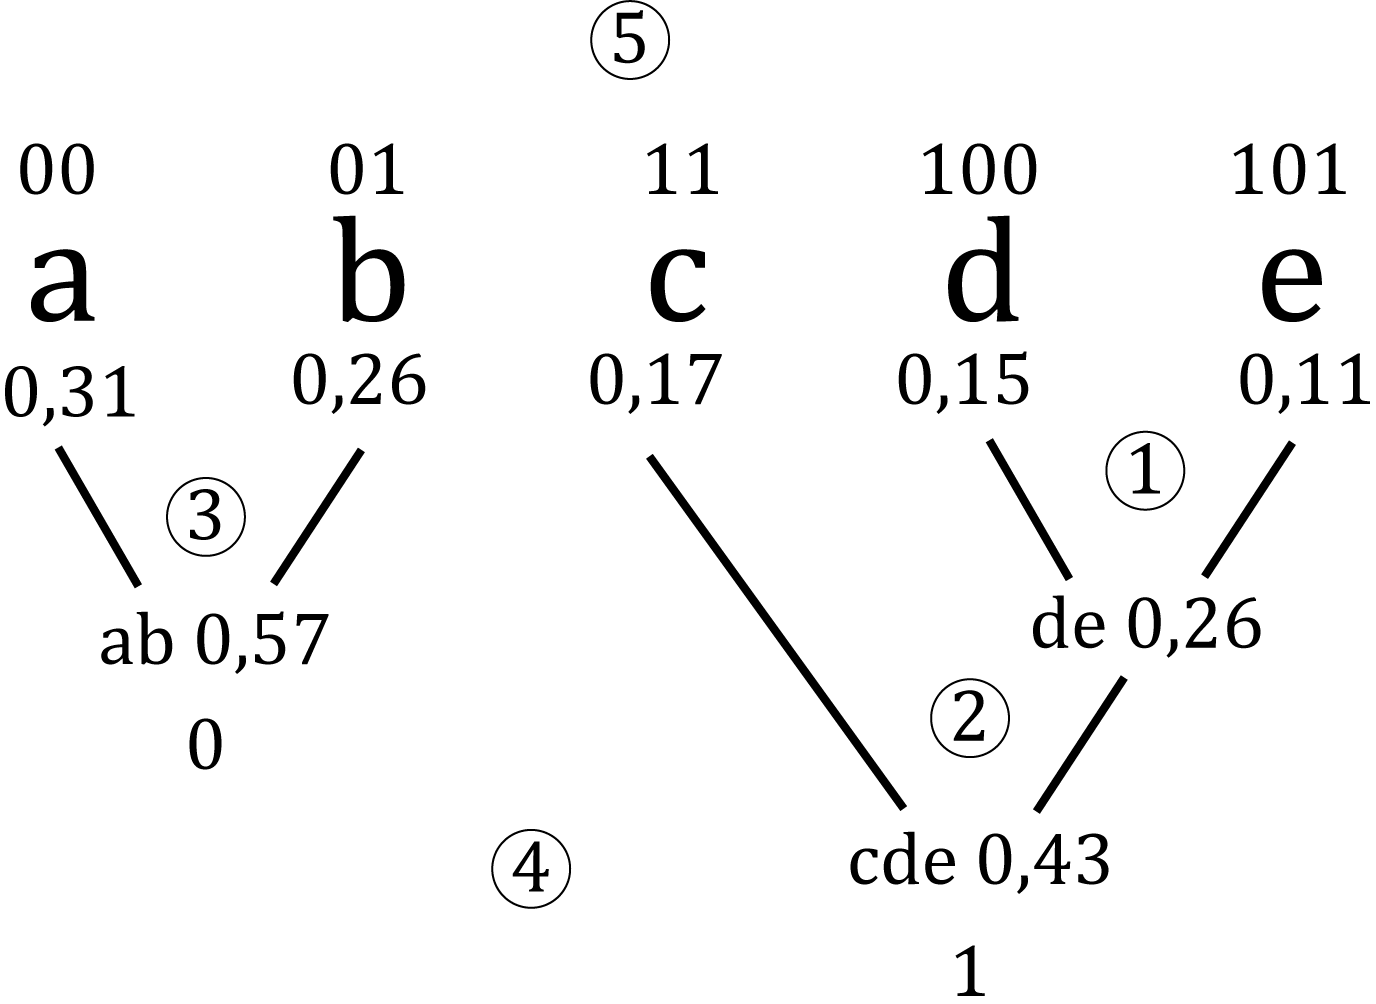
\includegraphics[width=5cm]{pics/25_1.png}
        \centering
    \end{figure}
  \end{example}
\end{document}
